\section{Analysis}
\label{sec:analysis}
\FloatBarrier

\begin{table}[t]
  \centering
  \caption{The variant grid: zero-shot top-1 (\%) with high-win-rate
  players, point estimates (per-cell 95\% CI half-widths are
  ${\sim}\pm0.1$--$0.2$pp on the dev sets, Table~\ref{tab:main};
  paired-difference CIs accompany the deltas in the text). A-noctx,
  A-proportional, and A-topfilter are architecture variants tested
  against the Full baseline before the deployed architecture was fixed.
  A-notext and A-noUB are the two pre-registered comparisons
  (\S\ref{sec:protocol}) analysed below: A-notext drops the 384-d text
  embedding from the Full recipe, and A-noUB removes the three
  licensed-IP training sets from A-noctx (the winning architecture,
  \S\ref{sec:arch}), so its clean comparator is the A-noctx row, not
  Full. The (variant $\times$ set) grid supplies the dev-side measurement
  of what the text embedding contributes on licensed-universe sets
  (per-set deltas below), computed before MSH is seen.}
  \label{tab:ablations}
  \small
  % AUTO-GENERATED by scripts/make_paper_tables.py -- do not edit.
% Pre-registered ablations (protocol section 5).
\begin{tabular}{lccccc}
\toprule
Variant & BRO & TMT & SOS & Dev mean & MSH \\
\midrule
Full (F-dev recipe) & 48.9 & 57.5 & 56.5 & 54.3 & \pendingcell \\  % run=20260704_135822_f_dev; run=20260704_135822_f_dev; run=20260704_135822_f_dev; run=20260704_135822_f_dev; pending: eval
A-notext & \pendingcell & \pendingcell & \pendingcell & \pendingcell & \pendingcell \\  % pending: BRO; pending: TMT; pending: SOS; pending: mean; pending: eval
A-noUB & \pendingcell & \pendingcell & \pendingcell & \pendingcell & \pendingcell \\  % pending: BRO; pending: TMT; pending: SOS; pending: mean; pending: eval
\bottomrule
\end{tabular}

\end{table}

\paragraph{Seed variance on the top-scoring variant.}
% Within-training top-1, not a dev-trio zero-shot re-eval: run=20260704_160422_a_noctx
% (0.6842), run=20260705_110803_noctx_seed18 (0.6803), run=20260705_133440_noctx_seed19
% (0.6796).
Two additional seeds of A-noctx (the recipe F-full uses, \S\ref{sec:arch})
land within-training top-1 at 0.680--0.684, a 0.5pp spread around the seed
reported in the table. So A-noctx's own accuracy is not a single lucky
initialization. But the margins between it and the neighboring
recipe-search variants are close (54.2--54.8 dev-mean,
Table~\ref{tab:ablations}), meaning the full ranking among variants has
not itself been seed-checked.

\paragraph{The flexibility-clause extras.} % run=20260705_220253_a_extras:
% BRO 0.4888 (CI 0.4878-0.4898), TMT 0.5758 (CI 0.5739-0.5776), SOS 0.5601
% (CI 0.5592-0.5611), dev-mean 0.5416, vs. A-noctx's 50.0/57.7/56.6/54.8.
% Paired-difference CIs (scripts/eval_ablation_deltas.py, evalproto.paired_
% bootstrap_diff, shared draft resamples, a_extras - a_noctx): BRO -0.0113
% (CI -0.0120,-0.0107), TMT -0.0015 (CI -0.0026,-0.0003), SOS -0.0057
% (CI -0.0062,-0.0052) -- all three exclude 0, so all three per-set deltas
% are real, not just the BRO one.
The protocol's flexibility clause (\S\ref{sec:protocol}) admits VOW
QuickDraft and the Powered Cube into F-full's training data only if a
dev-trio experiment shows a gain over A-noctx. Adding VOW QuickDraft to
A-noctx (same recipe and holdout, one shard added) scores 48.9/57.6/56.0,
dev-mean 54.2. That is lower than A-noctx's
\ANoctxBro/\ANoctxTmt/\ANoctxSos/\ANoctxDevMean{} on all three dev sets,
and the paired-difference CI excludes zero on every set ($-$1.1pp BRO, CI
$-$1.2 to $-$1.1; $-$0.1pp TMT, CI $-$0.26 to $-$0.03; $-$0.6pp SOS, CI
$-$0.62 to $-$0.52). So the clause's own rule excludes it: F-full's frozen
recipe (\S\ref{sec:arch}) does not train on VOW QuickDraft. The Powered
Cube half of the clause was not tested at all, since bulk per-pick data
for it is not available through the public \seventeenlands{} pipeline this
paper otherwise relies on exclusively, and acquiring it by another route
was out of scope. Both extras are therefore absent from F-full's training
data, one by a pre-registered result that failed to show a gain and the
other by an unmet data precondition, and the frozen recipe is exactly the
31-set corpus described in \S\ref{sec:data}.

\paragraph{What the text embedding contributes on licensed universes.}
MSH's names and flavor come from a comic universe, not from \mtg{}. Its
text lives in the sentence encoder's pretraining as a different genre.
This is the distribution shift most likely to break a text-dependent
model on the day it matters, which is why the protocol makes a
licensed-IP set (TMT) a development set: the rehearsal happens where it
can still inform design. One mitigation is built in: card names are
masked out of the text before embedding (\S\ref{sec:features}), so the
encoder sees mechanics, not franchises. A second design choice does not
reduce the shift but makes it measurable. The comparison grid of
Table~\ref{tab:ablations} separates what the text embedding contributes
on in-universe sets, SOS and BRO, from what it contributes on licensed
sets, TMT and MSH.

Zero-shot, the licensed dev set turns out not to be the hard one. TMT
reaches \FdevTmt\% against SOS's \FdevSos\% (and \RatioTmt\% vs
\RatioSos\% of their respective supervised references), which is
consistent with structured features carrying much of the load. The study
has no unmasked-text control, so it does not isolate name masking's effect.
The pattern could mean text adds little on licensed sets, or it could just
mean TMT is an easier format. The ablations provide association checks,
not a clean separation of those explanations:
% Arithmetic on Table~\ref{tab:ablations}'s own cells, both already
% run-tagged there: A-notext vs. Full (its comparator): BRO 48.9-45.8=3.1pp,
% TMT 57.5-55.9=1.6pp, SOS 56.5-53.1=3.4pp. A-noUB vs. A-noctx (its
% comparator per the table caption, not Full): BRO 50.0-49.2=0.8pp,
% TMT 57.7-57.5=0.2pp, SOS 56.6-54.9=1.7pp.
% Paired-difference CIs (scripts/eval_ablation_deltas.py,
% evalproto.paired_bootstrap_diff, shared draft resamples): text-penalty
% (Full - A-notext): BRO +0.0312 (CI 0.0304,0.0320), TMT +0.0159
% (CI 0.0146,0.0173), SOS +0.0342 (CI 0.0335,0.0349), dev-mean +0.0271.
% UB-penalty (A-noctx - A-noUB): BRO +0.0079 (CI 0.0072,0.0086), TMT
% +0.0021 (CI 0.0009,0.0033), SOS +0.0168 (CI 0.0162,0.0175), dev-mean
% +0.0089. All six per-set deltas exclude 0, including TMT's small 0.2pp
% UB-penalty (CI 0.09-0.33pp) -- pairing on identical held-out picks
% cancels enough between-draft variance that even this small a gap is
% distinguishable from noise, not just directionally suggestive.
dropping text costs TMT only \TextPenTmt pp (CI \TextPenTmtCi pp) against
its Full comparator, less than BRO's \TextPenBro pp (CI \TextPenBroCi pp)
or SOS's \TextPenSos pp (CI \TextPenSosCi pp). Text contributes least on
the sole licensed-IP development set, but that does not identify why.
Removing the three licensed-IP training sets from A-noctx changes BRO by
\UbPenBro pp (CI \UbPenBroCi pp), TMT by \UbPenTmt pp (CI \UbPenTmtCi pp),
and SOS by \UbPenSos pp (CI \UbPenSosCi pp). These paired differences are
statistically distinguishable from zero, but the ablation simultaneously
removes training volume, mechanics, and set composition. It therefore does
not identify a causal benefit of licensed-IP training. With one licensed
development set, the defensible conclusion is only that TMT did not expose
a transfer failure before the frozen MSH test.

\paragraph{Why BRO transfers worst.}
% scripts/eval_bro_transfer_analysis.py, run=20260704_135822_f_dev.
% Headline: BRO 0.4889, mean(TMT,SOS) 0.5701, gap 0.0812 (8.1pp).
% Bonus-sheet slice (BRR 63-card retro-artifact sheet, packs offering >=1
% bonus-sheet card vs. not): bonus_present top1 0.4062 (CI 0.4048-0.4077,
% n=510,654, 44.3% of picks), bonus_absent 0.5547 (CI 0.5535-0.5559,
% n=641,156). Raw gap 14.8pp. But has_bonus is a near-deterministic proxy
% for pick depth (BRO's booster carries exactly one BRR card per pack, so
% has_bonus falls monotonically from 100% at pick_number=0 to 2.9% at
% pick_number=14 (0-indexed; human picks 1-15); mean pick_number
% bonus_present=4.12, bonus_absent=9.28), and early picks
% are mechanically harder regardless of set. Stratifying by pick_number
% (weighted by bonus_present count per stratum, cluster-bootstrap CI over
% drafts): stratified gap 0.0307 (CI 0.0278-0.0336), i.e. ~80% of the raw
% 14.8pp is the pick-depth confound, not a bonus-sheet effect; the residual
% ~3.1pp is ~1.3pp (~16%) of BRO's 8.1pp shortfall against the trio, not
% "comparable in size to" it. Per-(pack,pick) curve: raw gap~pick_number
% corr 0.90 (widens through the pack), but lift-over-random-floor
% gap~pick_number corr -0.25 (narrows), reflecting BRO's 15-card vs.
% TMT/SOS's 14-card pack (pick_number 14 is a genuine BRO-only forced slot)
% rather than a real late-draft effect -- see Figure~\ref{fig:bro-diagnostics}.
BRO sits \BroTrioShortfall pp below the mean of TMT and SOS, at only
\RatioBro\% of its supervised reference. Of three candidate explanations, the bonus
sheet looked, at first pass, like the most direct: packs offering at
least one of the 63-card retro-artifact bonus sheet score
\BonusPresentTopOne\% zero-shot, while packs that don't score
\BonusAbsentTopOne\%, a \BonusRawGap pp raw gap on \BonusPresentFrac\% of
BRO's picks.

That gap turns out to be mostly a different artifact in disguise. BRO's
booster carries exactly one bonus-sheet card, so a pack can only ``have
the bonus card'' before it has been picked away. By construction,
\emph{has\_bonus} falls from 100\% at pick 1 to 2.9\% at pick 15 (BRO's
last, forced pick): bonus-present packs average pick 4.1, bonus-absent
packs average pick 9.3, and early picks are mechanically harder regardless
of what the pack contains. Stratifying by pick number before comparing
(Figure~\ref{fig:bro-diagnostics}) collapses the gap to \BonusStratGap pp
(CI \BonusStratGapCi), roughly 16\% of BRO's shortfall against the trio,
not something comparable in size to it.

The per-(pack, pick) curve shows the same family of artifact playing out
differently. The raw BRO-vs-TMT/SOS gap widens through the pack, but
BRO's booster carries one more card than TMT/SOS's (a real extra forced
pick, itself a consequence of the bonus sheet enlarging the pool), so
late raw picks are not apples-to-apples across sets. Correcting for the
random floor at each pick reverses the trend. Artifact-heavy color-signal
weakening and 2022-era recency remain plausible explanations but are not
separately isolated by this grid. With the bonus-sheet slice's real
contribution now measured at ~16\%, rather than assumed to explain most
of the shortfall, more of BRO's gap is left for those factors, and for
anything else this grid does not cover, to account for.

\begin{figure}[t]
\centering
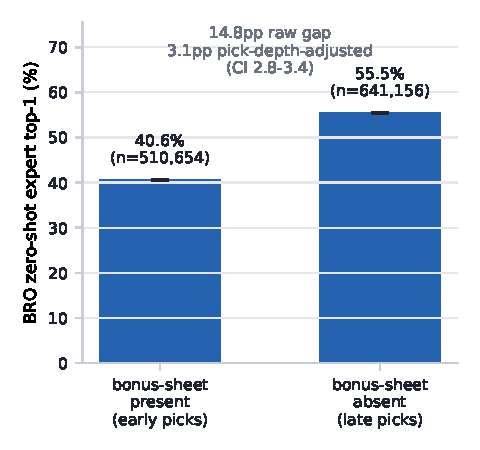
\includegraphics[width=0.55\linewidth]{figures/bro_diagnostics.pdf}
\caption{BRO zero-shot top-1 with high-win-rate players, split by whether
the pack offered at least one of the 63 BRR retro-artifact bonus-sheet
cards (\BonusPresentFrac\% of BRO's picks do). The raw \BonusRawGap pp
gap is mostly a pick-depth confound (labeled above the bars):
\emph{has\_bonus} tracks early-vs-late pick number by construction, and
stratifying by pick number before comparing collapses the gap to
\BonusStratGap pp (95\% CI). Error bars on the raw bars are 95\%
cluster-bootstrap CIs over drafts, computed from cached zero-shot
predictions.}
\label{fig:bro-diagnostics}
\end{figure}

\paragraph{Skill conditioning.}
Conditioning is a scorer-side input (\S\ref{sec:arch}), so one model
serves any audience. In human-model mode (\S\ref{sec:protocol}) the model
scores \FdevBroAllUsers\% / \FdevTmtAllUsers\% /
\FdevSosAllUsers\% on BRO / TMT / SOS: within a point of the
high-win-rate deployment numbers, consistent with skill moving picks
less than card quality does. Whether MSH shows the same pattern is a
question for the frozen pass (\S\ref{sec:msh}).

\begin{figure}[t]
\centering
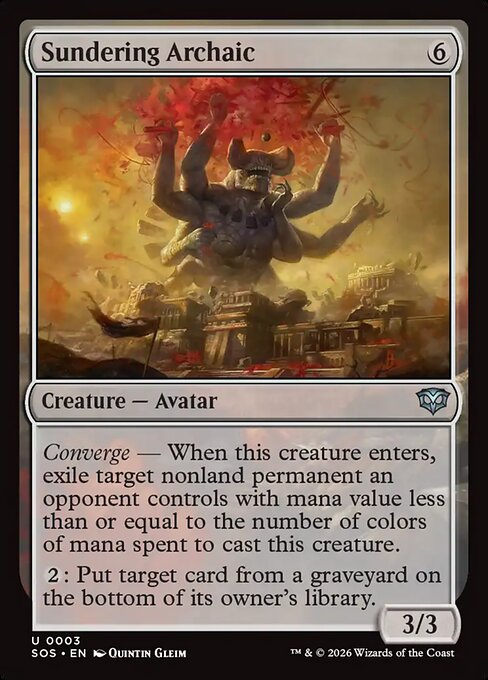
\includegraphics[width=0.12\linewidth]{figures/cards/sundering-archaic.jpg}%
\hspace{2mm}%
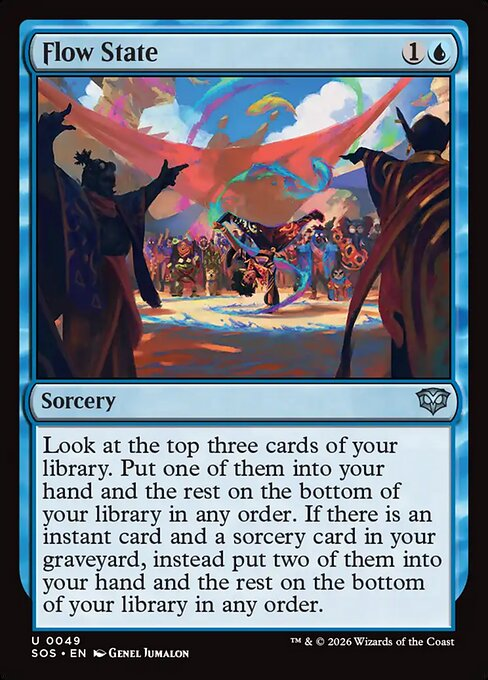
\includegraphics[width=0.12\linewidth]{figures/cards/flow-state.jpg}
\caption{The low-conviction end of the model's output: an illustrative
thirteen-card SOS pack (empty pool) where \VCCNameA{} and \VCCNameB{} score a near-exact
tie (EV \VCCEvA{} vs.\ \VCCEvB, dominance split \VCCSplitA/\VCCSplitB) --
the third candidate, \VCCRunnerName, trails at \VCCRunnerPct\% dominance
against the pair. Ties this close are exactly the regime the top-label ECE
below is measuring: the model's stated confidence and its actual
reliability at low conviction. Computed by the deployed per-set model.}
\label{fig:closecall}
\end{figure}

\paragraph{Calibration.}
% scripts/fit_dev_temperature.py, run=20260704_135822_f_dev. T=1 parity
% check against the published per-set ECE macros passed exactly before
% any T was chosen. Grid 0.30:3.00:0.02; frozen T selected by argmin mean
% dev-trio log-loss (Guo et al. 2017 convention), not ECE directly (ECE-
% argmin lands at T=1.40, mean ECE 0.0133, ~2x lower than the log-loss
% choice's 0.0250 -- so this leaves ECE on the table by design: log-loss is
% the smooth, proper scoring rule this protocol's other dev decisions
% already prefer, chosen over directly optimizing the number quoted in
% the text). Frozen into
% experiments/frozen_battery.json's "calibration" block before T0, applied
% to both deployment and human mode.
Zero-shot confidence falls well short of within-set calibration. Top-label
ECE is \FdevBroEce{} / \FdevTmtEce{} / \FdevSosEce{} on the dev trio,
against \CeilSosEce{} for the within-set SOS reference: roughly a five- to
seven-and-a-half-fold gap. The protocol permits one calibration decision: a
temperature fitted on dev only and frozen into the battery, never fitted
on MSH. That temperature is \FrozenTemperature, chosen by minimizing mean
dev-trio log-loss over a grid rather than ECE directly, since log-loss is
the smooth, proper scoring rule this protocol's other dev decisions
already use. It cuts the dev-trio mean ECE from \DevMeanEceAtTOne{} at the
unscaled T=1 to \DevMeanEceAtFrozenT{}, closing most of the gap above.
This temperature is fit on the logits of F-dev, the architecture-search
model that still has the set-context tower (\S\ref{sec:arch}), and applied
unchanged at test time to F-full, the tower-free recipe that actually
scores MSH. F-full has no held-out set of its own to fit a temperature
against without touching MSH, which is why the temperature crosses
architectures this way. How that crossed-over temperature fares on MSH
itself is reported with the frozen results (\S\ref{sec:msh}).

\paragraph{Late-draft retention.}
% scripts/eval_late_draft_retention.py, run=20260704_135822_f_dev, picks
% pack/pick-indexed >= 7 (0-indexed) vs. the per-set ceiling's own late
% picks. late_draft_retention: BRO 0.8180, TMT 0.8784, SOS 0.8925, dev-mean
% 0.8630 -- all higher than the corresponding overall (all-pick) ratios
% (0.745/0.810/0.805, dev-mean 0.787). Per-(pack,pick) curve: minimum
% margin (zero-shot top1 - random floor) over every non-forced-pick cell
% is 0.205 (BRO), 0.325 (TMT), 0.284 (SOS).
% Confound check (expert-slice zeroshot parquets, same run, computed
% directly from pack_size/target_rank, no new script): forced-pick rate
% (pack_size==1) at late picks vs overall -- BRO 0.1248 vs 0.0665, TMT
% 0.1435 vs 0.0735, SOS 0.1428 vs 0.0714 (roughly 2x). Mean pack_size late
% vs overall -- BRO 4.50 vs 8.01, TMT 3.98 vs 7.30, SOS 4.00 vs 7.50.
% Genuine (non-trivial, pack_size>=4) late top-1 vs overall top-1 -- BRO
% 0.4536 vs 0.4889, TMT 0.5397 vs 0.5750, SOS 0.5609 vs 0.5652: BELOW
% overall on all three, opposite of the raw retention ratio's direction.
Later picks are where a set-agnostic model could plausibly collapse to
rate-the-card, since pool signal has taken over from the card alone. The
pre-registered statistic, late-draft retention (\S\ref{sec:protocol}), is
\LateRetBro\% / \LateRetTmt\% / \LateRetSos\% on BRO / TMT / SOS (dev-mean
\LateRetDevMean\%), higher, not lower, than the corresponding all-pick
ratios (\RatioBro\% / \RatioTmt\% / \RatioSos\%, \S\ref{sec:results}). That
raw ratio is not, on its own, evidence that the pool tower is adding
signal late. Picks 8+ carry roughly twice the forced-pick rate of the
draft as a whole (forced picks score 1.0 by construction on both sides of
the ratio) and a substantially smaller mean pack size (4.0--4.5 cards
vs.\ 7.3--8.0 overall). Restricting to genuine choices, pack size $\geq$
4, excluding the trivial tail, puts late-pick top-1 \emph{below} the
all-pick figure on all three dev sets, the opposite direction from the
retention ratio. The claim the data does support is narrower: the model
does not collapse to chance late in the draft. The per-(pack, pick) curves
against the per-cell random floor show this directly, and
Figure~\ref{fig:pick-curves} in \S\ref{sec:msh} plots them for all four
sets. Excluding forced picks, zero-shot top-1 never comes closer than
20.5 (BRO) / 32.5 (TMT) / 28.4 (SOS) percentage points to chance at any
point in the draft, including its latest picks.
